\chapter{社会科学的研究设计}

\section{找准选题}

\subsection{导言}

在网上冲浪时,我们常常见到如下的讨论:

\begin{quote}
	{\fangsong 张三:某大学发表高水平论文证明了低收入人群喜欢吃辣。
	
	李四:***不是常识吗?这些学者\ldots\ldots(此处省略不文明用语)
	}
\end{quote}

作为社会科学的研习者,我们当然不会对研究意义产生虚无主义的印象,但一个不容忽视的问题的确摆在人们的面前,当前的社会科学界终于是陷入到一种为了``规范化''而``规范化''的境地,在学界``内卷''的体系之外,社会大众的评价似乎变得不再重要,研究的价值往往脱离现实。

这一点在量化研究之中的``显著性''和``稳健性''两大概念中体现得最为明显(简单理解即越显著越稳健越好),一些论文通篇粗制滥造,却执着于在量化部分雕花:你有一颗星显著(经济学认为此时犯错误的概率不超过百分之十),我就要有三颗星(不超过百分之一);你用一个稳健性证明了你的结论可靠,我就拉来十个证明结论稳健性的方式,做完后发现只有三种方式做出来可以接受(也就是至少有``一颗星''),那就专门把这三个放在上面。

于是最终呈现给外行人的结果便是``学术狗屁'',即洋洋洒洒几十页,证明了一个凭借直觉或者有一点生活经验便可以得出的结论,且通常与迫切需要改善的社会现实并无干系,呈现出一种``garbage
in, garbage out''的状态。

\subsection{好问题的标准}

好的研究问题应当符合五个关键标准,这些标准共同构成了一个层次分明的``金字塔模型''\textsuperscript{\cite{1}}。

\begin{enumerate}
	\item
	问题必须从小切口的困境出发,聚焦具体现象而非宏大命题,你自己要能把握住而不是给别人画饼。
	\item
	问题需要与既有研究脉络形成对话,明确识别并填补学术空白,比如将普遍原理运用于中国实际。
	\item
	优秀的问题应当兼具理论野心与实践价值,能够通过小问题推动理论进步,同时回应现实关切。
	\item
	问题必须具有可执行性,与研究者的能力、时间和资源相匹配,避免好高骛远,若缺乏定量技能就应选择质性方法\textbf{(当然本文目的是为定量打基础,你不能放弃!!)}。
	\item
	真正的好问题应当能激发研究者持续的探索欲,形成自我解惑的内在动力,不能写出一个自己都不想阅读的作品。
\end{enumerate}

按照三个层次区分并构成的完整的评价体系有:基础层要求具体可操作,中间层强调学术对话与创新,顶层注重理论与现实的平衡。需要牢记的是,提出好问题只是研究的起点,更重要的是通过扎实的方法论和持续努力将其转化为有价值的学术成果。

\subsection{寻找好问题}
本部分参考《政治学与公共管理研究方法基础》:\textsuperscript{\cite{2}}

要找到真正有价值的研究问题,首先需要明确研究目的,即这项研究究竟要解决什么问题、达到什么目标。

研究目的通常包含研究背景和研究意义两个核心维度。研究背景可以从时代背景和理论背景两个层面进行阐述。时代背景关注的是现实社会中的重大议题,通常体现为重要政策文件、关键会议精神或领导讲话要点,这些因素往往决定了研究的现实紧迫性。理论背景则需要梳理学科发展的脉络,既要关注经典著作中的核心观点,也要把握近期学术热点和前沿动态,这样才能找准研究的理论定位。

研究意义则可分为学术意义和实践意义两个层面。学术意义主要体现在对学科理论体系的补充、完善或创新,能够推动学科知识边界的拓展。实践意义则强调研究成果对现实问题的解释力、预测力或解决能力,能够为政策制定、社会实践提供科学依据。

研究问题的形成是一个动态的思维过程,通常需要经历探索和评价两个关键阶段。在探索阶段,研究者需要通过多种途径激发问题意识:

\begin{itemize}
	\item
	\textbf{系统地苦读文献}可以帮助研究者掌握学术脉络,发现已有研究的不足或空白。
	\item
	\textbf{深入体会现实}则要求研究者保持对实际问题的敏感度,从社会现象中提炼科学问题。
	\item
	\textbf{广泛与人交流}能够碰撞思想火花,不同学科背景的对话常常能催生创新视角。
	\item
	\textbf{学术顿悟}则是在长期积累基础上产生的灵感突破,往往能带来研究视角的重大转变。
\end{itemize}

在评价阶段,研究者需要建立严格的问题筛选标准,帮助我们逐步排除``灵光乍现''但``鸡肋''的问题。

\begin{itemize}
	\item
	\textbf{真实性}问题要求研究问题必须来源于客观现实或理论矛盾,而非主观臆测。
	\item
	\textbf{重要性}标准衡量问题的学术价值和社会影响。
	\item
	\textbf{善意原则}强调研究应具有建设性,避免无意义的争议。
	\item
	\textbf{明确性}要求问题表述清晰准确,避免模糊不清。
	\item
	\textbf{聚焦性}意味着问题范围要适中,既不过于宽泛也不过于狭窄。
	\item
	\textbf{有趣性}标准关注问题的创新性和吸引力,能够激发研究热情。
	\item
	\textbf{可操作性}则评估研究问题在现有条件下的可行性。
	\item
	\textbf{简洁性}强调问题的表述要精炼,避免冗长复杂。
\end{itemize}

选择研究问题的策略主要有两种典型路径,研究者可根据自身条件和研究目标灵活选择:

\begin{itemize}
	\item
	\textbf{扩散型问题}选择强调从核心问题向外拓展,适用于理论验证或应用推广类研究。这种方法需要严格遵循科学研究的规范流程,例如通过多案例比较来验证理论的普适性,或者采用不同方法进行稳健性检验以确保结论可靠。
	\item
	\textbf{漏斗型问题}选择则采取由面到点的思路,适用于复杂问题的逐步解析。这种方法的关键在于将宏大课题分解为若干可操作的子问题,通过层层递进的方式逐步深入。可以先界定核心概念,再分析影响因素,最后构建理论模型。这种化整为零的策略能够降低研究难度,提高可行性。两种方法各有优势,扩散型更注重结论的广泛适用性,漏斗型更强调研究的深度挖掘。
\end{itemize}

在实际研究中,两种思路往往需要交替使用,\textbf{初期可采用漏斗型方法聚焦核心问题,后期则可运用扩散型方法验证研究结论}。研究者应根据课题特点、自身专长和资源条件,选择最适合的问题切入路径。

\section{理论构建}

\subsection{概念、构念和理论}

本部分参考《政治学与公共管理研究方法基础》和《学术祛魅》\textsuperscript{\cite{3}}

\paragraph*{概念}

对客观现象的主观抽象,通过归纳同类事物的共同属性而形成,概念通常以字词或符号呈现,包含名词、内涵、指标和外延四要素,其中内涵的多维度需通过指标测量。清晰界定概念是理论建构的基础,其价值取决于三个因素:经验事实的支持、定义的精确性,以及与理论体系及其他概念的相关性------即该概念在理论解释中的必要性。例如《现代汉语词典》对``研究生''的定义即提炼了各类研究生的共性,如下:

\begin{quote}
	{\fangsong 大学本科毕业(或具有同等学力)后经过考试录取,在高等学校或科学研究机构学习、研究的学生。一般分为硕士研究生、博士研究生两级。有时特指硕士研究生。
	}
\end{quote}

\paragraph*{构念}

在研究的概念化过程中,明确区分\textbf{概念(concept)}和\textbf{构念(construct)}至关重要。

\textbf{概念}是指我们试图理解的抽象对象或现象本身,通常是研究需要测量的核心目标。而\textbf{构念}则是为了研究和测量这个抽象概念,人为建立的结构化表达形式,可以理解为该概念的\textbf{多个维度或侧面}。尤其在社会科学的领域中,所研究的概念往往复杂且难以直接捉摸,远不如自然科学中许多可以直接观测的对象那么直观,因此更需要深入细致地剖析。

为了更精确地理解和使用构念,我们可以对其进行分类分析。一个关键的分野是区分\textbf{显在构念}和\textbf{潜在构念}。\textbf{显在构念}指那些相对外在、可直接观察或测量(如用具体仪器)的属性。而\textbf{潜在构念}则隐藏于内,无法直接观测,需要通过间接手段来衡量。有些潜在构念(如身高、体重)虽然存在于物理或生理层面,相对容易通过标准工具测量;然而,更多在社会科学中关心的潜在构念(如自尊、魅力、社会凝聚力等)则具有高度的主观性和抽象性,它们无法被直接``看到''或``摸到'',往往只能通过人们的\textbf{感知、陈述或行为表现}来推断。这使得这类构念带有一种``\textbf{只可意会,难以言传}''的特性。正是由于社会科学研究的核心对象多是这种复杂的潜在构念,研究者必须精心设计和运用各类问卷、量表、行为观察或其他策略化工具,才能有效地触及和测量我们真正关心的深层概念。

一句话总结便是:概念要想落地,就需要找到概念指涉事物本身的共性加以把握,构念就是操作化的前瞻,也是找寻变量的开端。

\paragraph*{理论}

描述的是概念间关系,其定义有如下几个表述:

\begin{quote}
	{\fangsong 《现代汉语词典》强调理论的实践性、知识性和系统性;《美国传统辞典》侧重解释功能、可检验性和预测性;默顿关注逻辑命题和经验一致性;艾尔·巴比突出对事实规律的解释;巴卡拉克强调概念变量系统;特纳注重观念性和解释功能;范埃弗拉提出理论包含因果规律等要素。
	}
\end{quote}

综合来看,理论是人类基于实践或研究形成的系统性、可检验的知识体系,用于描述、解释和预测自然或社会现象,包含概念、变量、机制、命题等要素。

近年来较为``出圈''的中层(中观)理论(默顿),以及一些广为人知的宏观微观理论也分别有一些定义和解释:

\begin{itemize}
	\item
	\textbf{宏观理论}:高度抽象复杂,解释世界本质和基本规律,如相对论、马克思主义、结构功能主义等。
	\item
	\textbf{中观理论}:介于两者之间,研究特定现象或群体,如公共资源治理理论、国家理论等。
	\item
	\textbf{微观理论}:聚焦具体概念关系,由可验证的命题构成,如少婚导致少子之类的简单判断。
\end{itemize}

检验理论离不开操作化的环节,需要明确的是,操作化的目的不是为了证明``先验''理论的正确,即不能带着答案找问题。

\subsection{操作化}

\paragraph*{变量(variable)}


又称为变项,是对概念内涵操作化和具体化的产物。变量,顾名思义,即变化的量,是具有一个以上不同取值(不同的子范畴、不同的属性,或不同的亚概念)的概念。至于只有一个固定值的概念,则称为常量。举例而言,``性别''这一变量就包括了``男性''与``女性''两个不同的子范畴;``受教育水平''这一变量就可以分为``小学及以下''\,``初中''\,``高中''\,``大学本科或专科''\,``硕士研究生''\,``博士研究生''六个不同子范畴;工资收入更是有诸多取值可以填写。


在科学研究中常常使用变量语言及变量思维来描述或解释研究现象之间的关系。变量的使用是为了观测概念,亦是为了通过探寻变量间的关系,更便利地研究不同概念间的关系。将概念具体化为可以测量的变量,并说明不同变量以及变量的不同属性(属性就是事物的本性或特征)之间的逻辑关系,是建构理论的关键环节。

\paragraph*{变量间关系}

在科学研究中,能够产生新的理论贡献是学术界一直以来的期望,这就要求研究者对变量的选择及其关系做出理论说明。在建立理论的过程中,变量之间并不是孤立的、割裂的,而是存在着某种逻辑关系,一般情况下存在以下三种关系来解释变量间的机制或原理:

\begin{itemize}
	\item
	\textbf{直接关系},即那些用箭头把两个概念直接连在一起的图形所表示的关系,如X→Y,这表示变量X与变量Y之间存在着直接效应。
	\item
	\textbf{间接关系(中介关系)},即包含中介链的关系。比如变量X对变量Y的效应被认为是通过一个中间变量Z来产生的,我们就把变量Z称为中介变量,它们之间的关系表示为X→Z→Y。
	\item
	\textbf{调节关系},指的是自变量和因变量的因果关系机制中包含有调节变量的关系。需要注意的是,调节变量调节的是一个关系,而不是一个变量,如果用图形表示,调节变量调节的是X→Y中间的``→''。
\end{itemize}

\begin{figure}[htbp]
	\centering
	\fbox{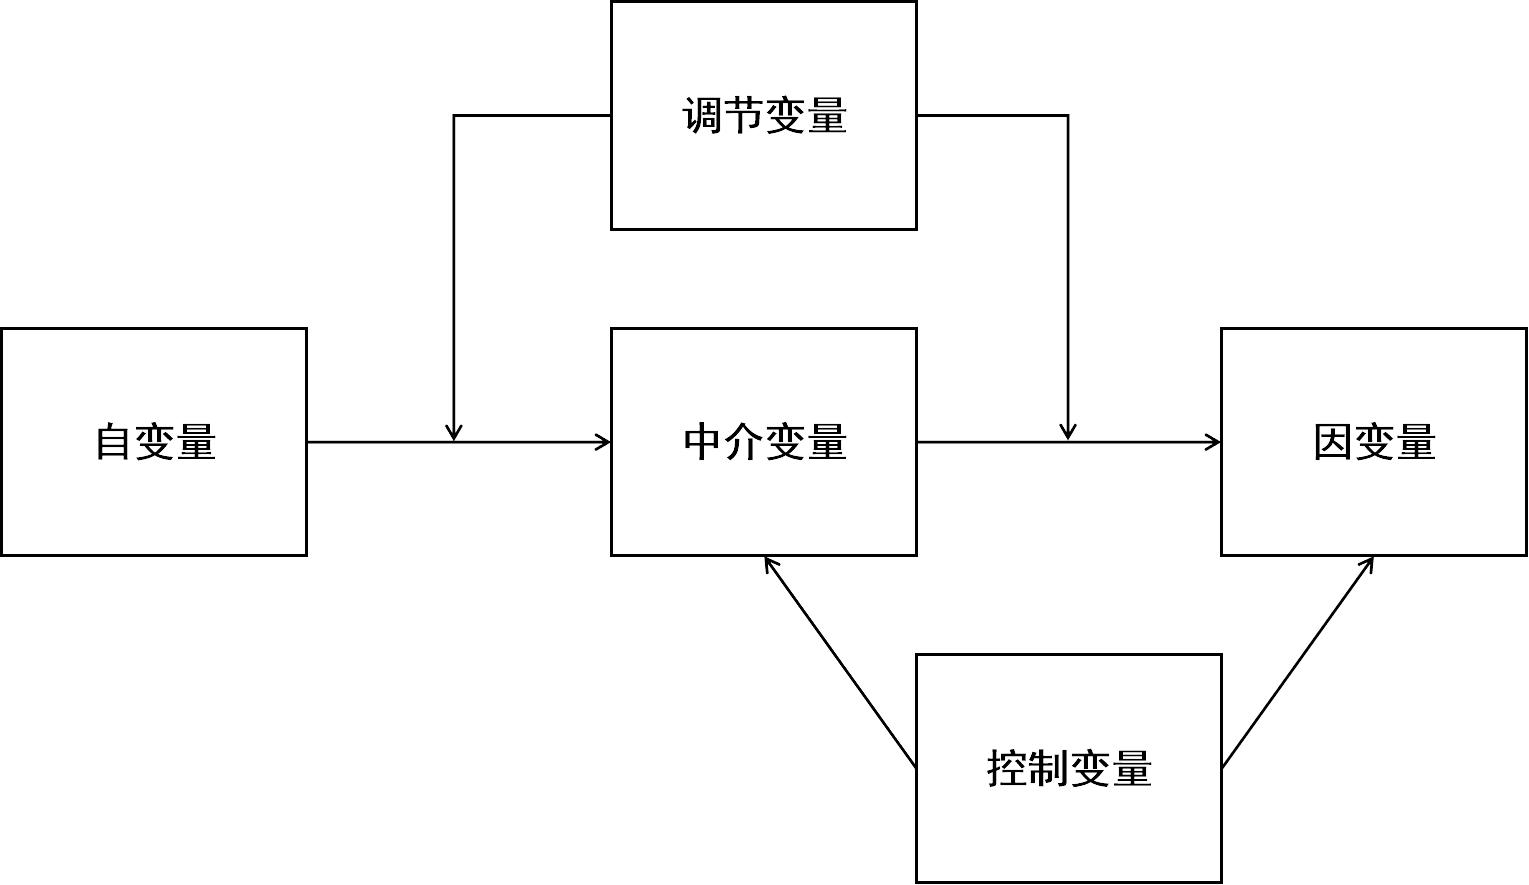
\includegraphics[width=0.5\textwidth]{image/f1.jpg}} % 用 \fbox 包裹图片
	\caption[变量间关系]{变量间关系}
	\label{fig:relation}
\end{figure}

需要明确的是,并非只有量化分析才需要用到变量思维,当代的政治科学名著中,如亨廷顿《变化社会中的政治秩序》,尽管没有用明确的假设H1一类指出,更没有用到统计分析,却仍然有一个完整的链条,总结一下大约是:

\begin{itemize}
	\item \textbf{自变}量:政治权威。
	\item \textbf{因变量}:政治发展。
	\item \textbf{中介变量}:政治秩序。
	\item \textbf{调节变量}:政党、领导人、社会结构等等。
	\item \textbf{控制变量}:一国的历史与现在(国家异质性)、国际体系变化等等。
\end{itemize}

\paragraph*{命题(proposition)}

是``对于一个概念的特征或多个概念间关系的陈述''。例如,``受教育水平更高的人相较于受教育水平更低的人文化消费更多''。

\paragraph*{假设(hypothesis)}

是命题的一种特殊形式,是为了得到逻辑的或经验的结论并加以检验而做的尝试性假说。假设通常是试探性的(也可以理解为实验性的),是为了被检验的目的而提出的严格的假设或建议。从这个角度来说,研究者通过提出待检验的假设,在抽象理论与经验事实之间建立了联结。

在大多数的社会科学研究中,由于研究者的主要目的大都可以归结为解释或说明不同变量之间的因果关系,因而,提出和检验有关变量间关系的假设成为科学研究和理论建构中不可或缺的环节。一般而言,假设有以下三种陈述方式:

\begin{itemize}
	\item
	\textbf{条件式陈述(conditional
		statement)}:其表达形式为``如果x,则y'',其中x代表前提或先决条件,y为结果。这种方式通常表示两个变量之间存在因果关系,但有时也指代相关关系。
	\item
	\textbf{差异式陈述(differential
		statement)}:其表达形式为``A组与B组在变量x上无(或有)差异''。在统计学中,无差异假设即``零假设''或``虚无假设''。
	\item
	\textbf{函数式陈述(functional
		statement)}:其数学表达式为y=f(x),即y是x的某种函数。它说明,如果变量x发生变化,则y也相应发生变化,反之亦然。函数式陈述在自然科学研究中较为常见,在以因果推断为方向的社会科学中也有增加的趋势。
\end{itemize}

\section{具体方法}

\subsection{研究对象}

\paragraph*{研究对象的选择与界定}

在开展研究时,明确研究对象是至关重要的第一步。研究对象的核心在于确定\textbf{分析单位},即研究的基本观测点。常见的分析单位包括:

\begin{enumerate}
	\item
	\textbf{个体层面}:以个人为研究对象,例如研究``个人收入差异的影响因素'',分析教育程度、工作经验等对个体收入的影响。
	\item
	\textbf{组织层面}:以企业、学校等组织为对象,比如探讨``企业创新效率的决定因素'',考察研发投入、人才结构等组织特征的影响。
	\item
	\textbf{国家层面}:以国家或地区为分析单位,如比较``不同产业政策对经济增长的影响'',需要收集各国政策和经济数据。
\end{enumerate}

需要警惕的是\textbf{生态学谬误},即错误地将高层次的分析结论直接推论到低层次单位。例如,用国家层面的收入不平等数据来推断个体幸福感,就可能犯这种错误——相对剥夺理论的最初研究就踏入其中\textsuperscript{\cite{4}}。

\paragraph*{数据类型}

研究设计时还需考虑\textbf{时空维度}的选择:

\begin{itemize}
	\item
	\textbf{截面数据}:捕捉同一时间点不同地区的状况,适合进行横向比较。例如2023年各省教育投入比较。
	\item
	\textbf{时序数据}:追踪同一地区不同时间的变化,适合趋势分析。如某省2000-2023年教育投入增长。
	\item
	\textbf{面板数据}:兼具截面和时序维度,能同时分析地区差异和时间变化。如全国31个省区市2010-2023年的教育投入数据。
\end{itemize}

\subsection{获取与分析数据}

找准所需数据的类型后,进入到数据分析方法的环节,以教育为主题为案例举例分析:

\paragraph*{观察法}

指研究者通过系统观察并记录教学过程中的现象来收集数据。例如,要研究教师提问方式对学生课堂参与度的影响,研究者可以在课堂上记录教师提问的类型(如开放式问题或封闭式问题)以及学生的回应情况(如举手次数、回答质量)。这种方法适用于自然教学环境下的行为研究,但存在两个主要挑战:一是观察者可能因主观判断产生偏差,二是若观察的课堂样本不足或仅限于特定班级,可能导致结论缺乏普遍性。

\paragraph*{实验法}

通过主动干预来验证教学方法的因果效应。典型操作是将学生随机分组,对实验组采用新教学方法(如项目式学习),对照组维持传统教学(如讲授式),学期末比较两组学生的成绩差异。例如,研究翻转课堂的效果时,随机分配部分班级使用课前视频学习+课堂讨论,另一部分采用常规授课,最终通过标准化测试评估学习成效。实验法的核心要求包括随机分组(确保学生基础水平均衡)、控制无关变量(如教材、课时一致),以及实验过程可重复验证。这种方法能直接证明教学方法的优劣,但可能因实验环境与真实课堂的差异而影响外部效度;在某些情况下,干预违背研究伦理而无法开展。

\paragraph*{准自然实验法}

当无法随机分组然后实验时,可利用教育政策或学校制度变化作为``自然实验''条件。例如,某地区推行``小班化教学改革'',研究者可比较改革前后同一学校学生的成绩变化,或对比改革校与非改革校的差异,使用双重差分法(DID)排除生源波动等因素干扰。另一种情况是,利用学校按分数线分班的规则(如``实验班''与普通班的分数线临界点),采用断点回归(RDD)分析教学差异对成绩的影响。这种方法依托现实教育场景,但需注意其他变量(如家庭支持、教师经验)可能混淆结论。

\subsection{总体与样本}

本部分参考《政治学与公共管理方法基础》,在讨论具体方法之前,我们需要明确几个核心概念:

\paragraph*{要素}

研究的基本分析单位,也是信息收集的对象,可以是一个人、一个班级、一所学校等。

\paragraph*{总体}

指研究对象的全部要素的集合,比如``某市所有高中生''就是一个总体。

\paragraph*{样本}

从总体中抽取的部分要素的集合,比如从该市随机选取的500名高中生。

\paragraph*{样本规模}

又称样本容量,指的是样本中包含的要素数量,比如上述的500人。

\paragraph*{样本代表性}

指样本在多大程度上能够反映总体的特征。一般来说,当样本的关键特征(如性别比例、成绩分布等)与总体越接近,代表性就越好。

\paragraph*{抽样}

无论选择哪种研究方法(质性研究还是量化研究),都要求我们从总体中抽取一定样本(否则真要累死),那具体怎么抽呢?抽样就是从研究总体中选择部分个体或要素作为样本的过程。要完成抽样,首先需要明确\textbf{抽样框}------也就是包含所有研究对象的清单或规则(比如全校学生名单),同时确定\textbf{抽样单位},即实际抽取的基本单位(比如个人、班级或学校)。

抽样方法主要分为两大类:\textbf{非概率抽样}和\textbf{概率抽样}。

\textbf{非概率抽样}不依赖随机原则,而是根据研究需求、主观判断或现实条件来选取样本,适合探索性研究或特殊案例分析。常见方法包括:

\begin{itemize}
	\item
	\textbf{方便抽样}:选最容易获取的样本(比如就近调查自己班的学生);
	\item
	\textbf{目标抽样}:按特定标准选取(比如只研究成绩前10\%的学生);
	\item
	\textbf{滚雪球抽样}:通过已有样本推荐新样本(比如通过少数留学生找到更多留学生受访者);
	\item
	\textbf{配额抽样}:按比例匹配总体特征(比如男女各抽50人);
	\item
	\textbf{典型案例抽样}(选最具代表性的案例)、\textbf{极端案例抽样}(选表现异常好或差的个体)、\textbf{负面案例抽样}(故意选不符合理论的案例)等。
\end{itemize}

\textbf{概率抽样}则严格遵循随机原则,确保每个个体有已知的、非零的被抽中概率,适合需要统计推断的研究。常用方法有:

\begin{itemize}
	\item
	\textbf{简单随机抽样}:像抽签一样完全随机选取;
	\item
	\textbf{系统抽样}:按固定间隔抽取(如每第10个学生);
	\item
	\textbf{分层抽样}:先按特征分组(如年级),再在各层内随机抽;
	\item
	\textbf{整群抽样}:随机抽取完整群体(如抽几个班级而非个别学生);
	\item
	\textbf{多阶抽样}:分多个阶段逐步缩小范围(如先抽城市,再抽学校,最后抽班级)。
\end{itemize}

\paragraph*{抽样误差}

抽样过程不可避免地会产生\textbf{误差},即样本统计量(如样本平均分)与总体参数(如全市高中生真实平均分)之间的差异。这种误差是随机产生的(\textbf{无法根除}),但可以通过科学的抽样方法和适当的样本规模来降低(\textbf{但不能躺平})。

选择抽样方法时,非概率抽样灵活但可能偏差大,概率抽样科学但成本高。实际研究中常结合使用,比如先滚雪球找到目标群体,再用分层抽样确保代表性。

\subsection{得出结论}

本部分参考《政治学与公共管理方法基础》、《比较政治学:理论与方法》\textsuperscript{\cite{5}}和《比较政治中的议题与方法》\textsuperscript{\cite{6}},为了确保我们得出的是一个流程科学结果合理的结论,我们还需要反复考量如下要求:

\paragraph*{控制变异}

在社会科学研究中,控制变异是确保研究结论可靠性的关键环节。研究者需要通过系统的方法来最大化研究变量的差异,控制干扰因素,并减少测量误差。

\begin{enumerate}
	\item \textbf{最大化系统差异}:指由于自变量变化而引起的因变量的变化幅度要达到最大(变化越大越能找到规律)。明确研究问题,确定最佳的自变量和因变量,同时应该考虑到自变量和因变量的所有情况,并选定合理的样本范围。
	\item \textbf{控制外生变量} :控制外生变量主要有三种方法:
	
	\begin{itemize}
		\item \textbf{纳入法}:将可能影响结果的重要变量纳入分析模型。\textbf{核心变量}(如政策实施年份、受教育年限)必须包含,同时要控制\textbf{人口统计学变量}(如年龄、性别)和\textbf{环境变量}(如行业类型、宏观变量等)。
		\item \textbf{非纳入法}:通过研究设计来控制变量。\textbf{同质法}即没有外生变量不一致导致的误差(一般这样只能找到有限个特征相同,不能保证完全相同,用得很少);\textbf{随机分配法}确保\textbf{实验组}和\textbf{对照组}在各方面均衡(概率抽样);\textbf{配对法}则根据相似特征(如经济发展水平、人口规模)来匹配比较对象。
	\end{itemize}
	\item
	\textbf{最小化误差差异}:测量误差的控制至关重要。采用标准化测量工具(如Likert五级量表)可以提高数据一致性。同时,通过多源数据交叉验证,也可以显著提升数据的准确性和可靠性。
\end{enumerate}

\paragraph*{研究效度}

\begin{itemize}
	\item
	\textbf{构念效度}:指一个构念能够正确反映其所要表达、描述或测量对象内容和特征的程度,或者也可以定义为一个构念表达、描述和测量的精确性。
	\item
	\textbf{内部效度}:指基于特定研究对象而得出的结论本身符合特定研究对象实际情况的程度;而对探求精确因果性关系的定量研究而言,则是基于特定研究对象得出的变量(或构念)间因果关系的推论符合特定研究对象实际情况的程度,也即其因果关系推论对特定对象本身而言的可信度。
	\item
	\textbf{外部效度}:指将从特定研究对象得出的研究结论推广到具有不同分析单位、时间维度、研究区域、研究层次、研究尺度等的其他研究对象的可信度。
	\item
	\textbf{统计结论效度}:指通过统计检验对假设关系进行解释的可信度。
\end{itemize}

需要说明的是,这四种效度常互相制衡(如提高内部效度可能损害外部效度);而追求统计结论效度实际上也可能犯了构念效度的损伤(试变量试到跑题)。

\section{定性与定量的融合}

上文虽然是定量分析的范式,但定性亦可参照一二,诸多时候定量分析的理论渊源实际上来自定性,更遑论KKV(加里·金/Gary King、罗伯特·基欧汉/Robert O. Keohane、悉尼·维巴/Sidney Verba)三人经典的《\emph{Designing Social Inquiry}》中早已有详尽的解释(其繁体版译本名为《好研究如何設計?:用量化邏輯做質化研究》)。

对这一部分的理解有助于我们理解计量经济学的开端、发展与变革,从而更好理解结构计量的设计转向。值得注意的是,KKV倡导的``量化逻辑''并非要将质性研究简单数字化,而是强调研究设计中的因果推断逻辑必须严谨。这种思想与Angrist等人提出的``可信性革命''遥相呼应,二者都要求研究者超越方法论的二元对立,在保持方法适切性的前提下实现优势互补。当处理异质性处理效应时,定性访谈揭示的个体决策过程往往能修正定量模型的设定偏误;而大样本数据分析又能检验质性研究发现的外部效度。

\newpage
\thispagestyle{empty}
\begin{thebibliography}{99}
	\bibitem{1}
	董晨宇 \ 等,《拆论文:从精读中领悟学术写作》,重庆大学出版社
	
	\bibitem{2}
	杨立华 \ 等,《政治学与公共管理研究方法基础》,北京大学出版社
	
	\bibitem{3}
	马亮,《学术祛魅:实证研究十讲》,中国人民大学出版社
	
	\bibitem{4}
	王正绪 \ 等,《比较政治学》,复旦大学出版社
	
	\bibitem{5}
	B.盖伊·彼得斯,《比较政治学:理论与方法》,上海人民出版社
	
	\bibitem{6}
	托德·兰德曼 \ 等,《比较政治中的议题与方法》,上海人民出版社
	
\end{thebibliography}